% Created 2023-09-20 mié 11:24
% Intended LaTeX compiler: pdflatex
\documentclass[11pt]{article}
\usepackage[utf8]{inputenc}
\usepackage[T1]{fontenc}
\usepackage{graphicx}
\usepackage{grffile}
\usepackage{longtable}
\usepackage{wrapfig}
\usepackage{rotating}
\usepackage[normalem]{ulem}
\usepackage{amsmath}
\usepackage{textcomp}
\usepackage{amssymb}
\usepackage{capt-of}
\usepackage{hyperref}
\usepackage{../modern}
\bibliography{./fuentes.bib}
\raggedbottom
\setcounter{secnumdepth}{2}
\author{Luis Eduardo Galindo Amaya (1274895)}
\date{17 de Septiembre 2023}
\title{Taller 2 Administración de archivos}
\hypersetup{
 pdfauthor={Luis Eduardo Galindo Amaya (1274895)},
 pdftitle={Taller 2 Administración de archivos},
 pdfkeywords={},
 pdfsubject={},
 pdfcreator={Emacs 27.1 (Org mode 9.3)}, 
 pdflang={Spanish}}
\begin{document}

\modentitlepage{../images/escudo-uabc-2022-color-cont.png}
\tableofcontents\pagebreak
\datasection{Individual}


\section{Introducción}
\label{sec:org2348f37}
En los sistemas operativos unix es esencial conocer como administrar archivos 
ya que esto nos permitirá aprovechar al máximo el sistema operativo, algunas 
de las acciones mas comunes son: copiar archivos, crear archivos, moverlos a 
los directorios y listar su contenido, a lo largo de este taller utilizaremos 
algunos commandos que nos proporciona el sistema operativo para lograr estos 
objetivos.

\pagebreak

\section{Actividades}
\label{sec:org8bd98df}
\subsection{Copie el archivo primero que está dentro de maestro/poesía a su home directory}
\label{sec:org52719f8}
\begin{verbatim}
cd ..
cp alma/filtros/amorosos galindo/
\end{verbatim}

\begin{figure}[htbp]
\centering
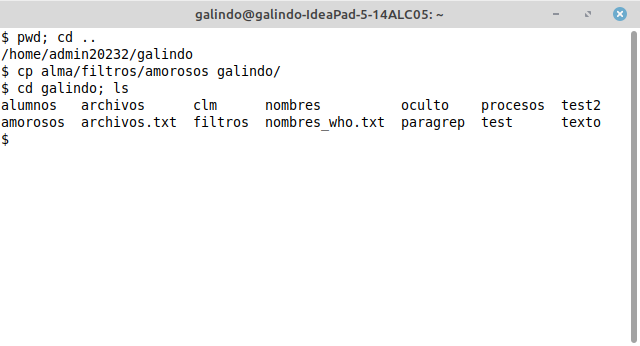
\includegraphics[width=10cm]{img/a1.png}
\caption{Archivo copiado en el directorio home}
\end{figure}

\subsection{Copie el archivo segundo (está en el mismo directorio) a su home directory}
\label{sec:orga0cfbd8}
\begin{verbatim}
cd .. 
cp alma/filtros/segundo galindo/
\end{verbatim}

\begin{figure}[htbp]
\centering
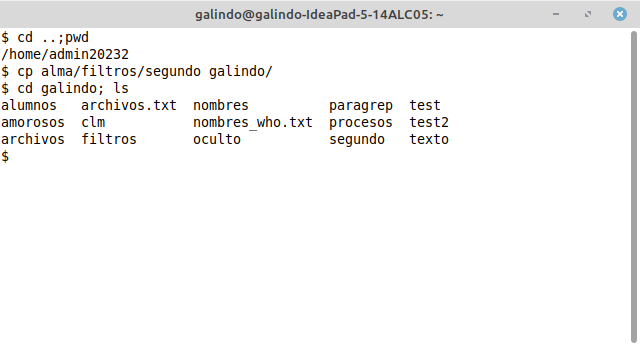
\includegraphics[width=10cm]{img/a2.png}
\caption{copiar segundo a mi directorio}
\end{figure}

\pagebreak

\subsection{Copie el archivo intermedio de maestro/poesia a su home directory}
\label{sec:org760ff7d}
\begin{verbatim}
cp ../alma/filtros/intermedio ./
\end{verbatim}

\begin{figure}[htbp]
\centering
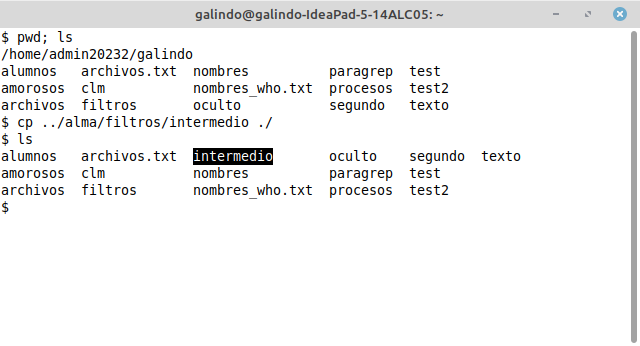
\includegraphics[width=10cm]{img/a3.png}
\caption{copiar intermedio a mi directorio}
\end{figure}

\subsection{Verifique el contenido de los tres archivos}
\label{sec:orgfa4a804}
\begin{verbatim}
cat amorosos
cat segundo
cat intermedio
\end{verbatim}

\begin{figure}[htbp]
\centering
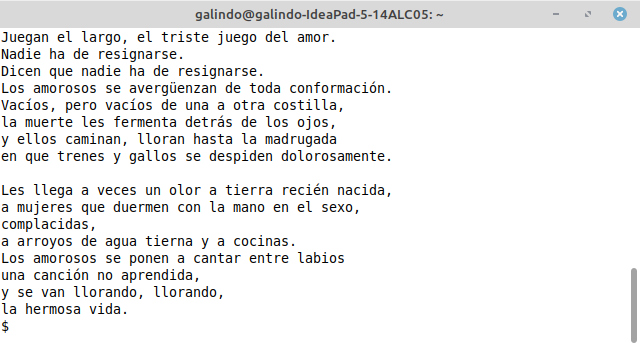
\includegraphics[width=10cm]{img/amorosos.png}
\caption[\texttt{cat amorosos}]{salida de \texttt{cat amorosos}}
\end{figure}

\begin{figure}[htbp]
\centering
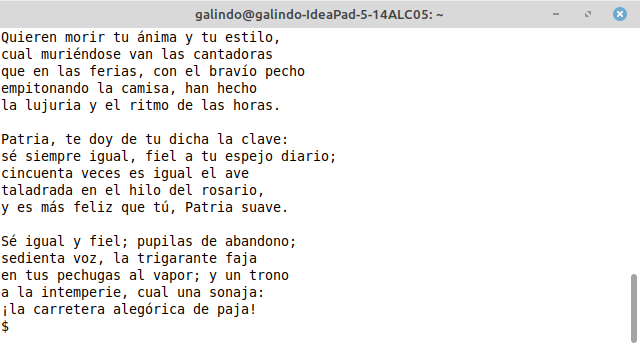
\includegraphics[width=10cm]{img/segundo.png}
\caption[\texttt{cat segundo}]{salida de \texttt{cat segundo}}
\end{figure}

\begin{figure}[htbp]
\centering
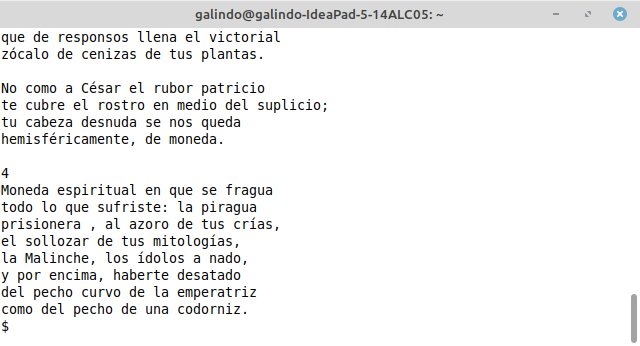
\includegraphics[width=10cm]{img/intermedio.png}
\caption[\texttt{cat intermedio}]{salida de \texttt{cat intermedio}}
\end{figure}

\cite{linux_cat}

\pagebreak

\subsection{Borre los tres archivos copiados en los pasos 2, 3 y 4}
\label{sec:orgf6946fa}
\begin{verbatim}
rm ~/primero ~/segundo ~/intermedio
\end{verbatim}

\begin{figure}[htbp]
\centering
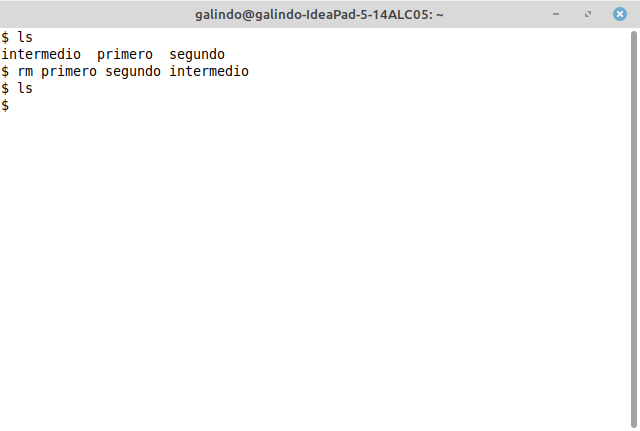
\includegraphics[width=10cm]{img/a5.png}
\caption{Archivo eliminados}
\end{figure}

\subsection{Copie los tres archivos (primero, segundo e intermedio) utilizando una sola instrucción}
\label{sec:org2606518}
\begin{verbatim}
cp ../alma/filtros/primero\
   ../alma/filtros/segundo\
   ../alma/filtros/intermedio\
   ./poesia/
\end{verbatim}

\begin{figure}[htbp]
\centering
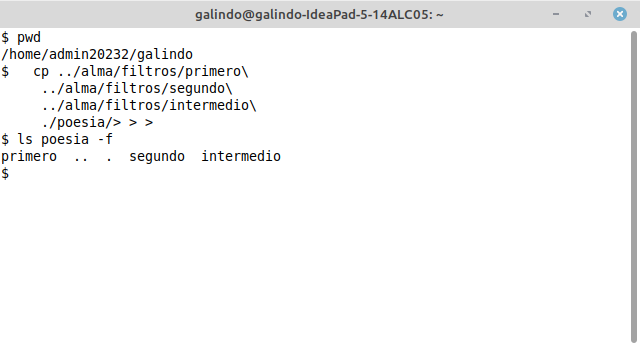
\includegraphics[width=10cm]{img/a6.png}
\caption{Listar los archivos en poesía}
\end{figure}

\subsection{Muestre en pantalla el contenido de segundo e intermedio usando una sola línea}
\label{sec:org4dcbdb8}
\begin{verbatim}
cat poesia/segundo poesia/intermedio
\end{verbatim}

\begin{twoc}
\begin{center}
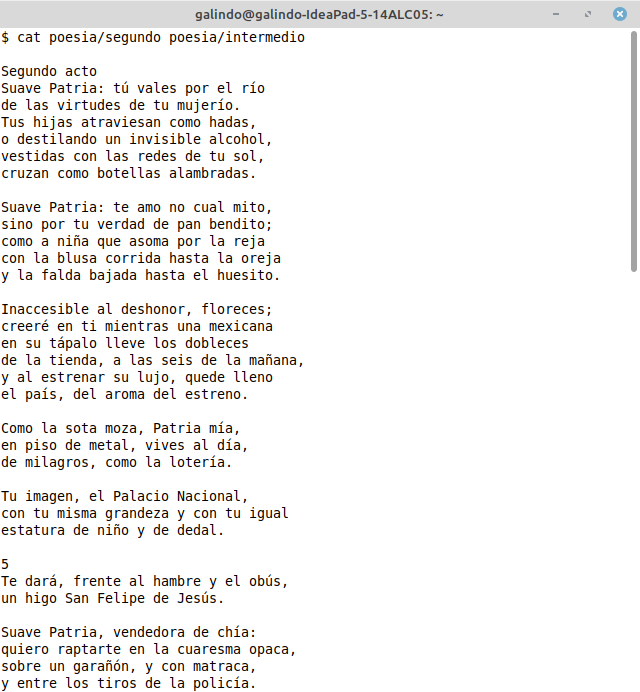
\includegraphics[width=.9\linewidth]{img/1.png}
\end{center}
\end{twoc}
\begin{twoc}
\begin{center}
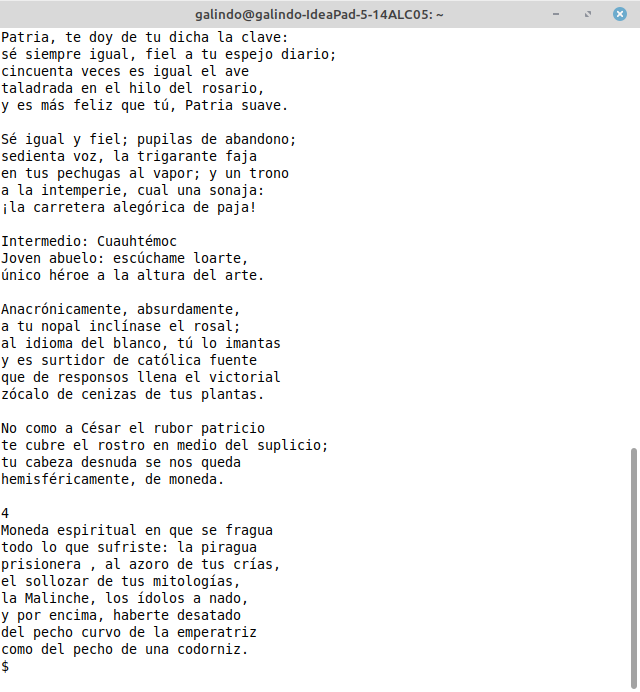
\includegraphics[width=.9\linewidth]{img/2.png}
\end{center}
\end{twoc}

\cite{linux_cat}

\subsection{Muestre en pantalla el contenido de Enpaz.txt, numerando cada línea}
\label{sec:org0c81fc1}
\begin{verbatim}
cat -n ../alma/filtros/Enpaz.txt
\end{verbatim}

\begin{figure}[htbp]
\centering
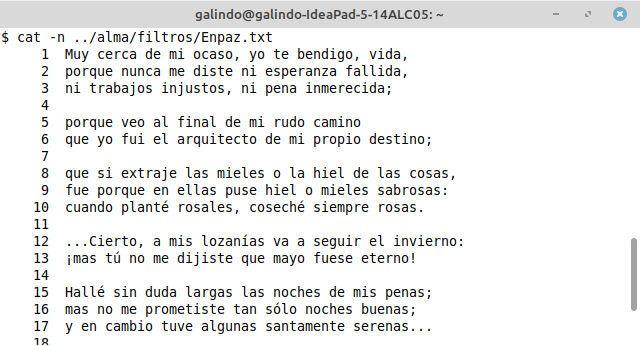
\includegraphics[width=10cm]{img/a8.png}
\caption[\texttt{cat -n ../alma/filtros/Enpaz.txt}]{Salida de \texttt{cat -n ../alma/filtros/Enpaz.txt}}
\end{figure}

\cite{linux_cat}

\pagebreak

\subsection{Copie el archivo SuavePatria.txt de maestro/poesia a su directorio de inicio y renómbralo como 'patria'}
\label{sec:org7f88729}
\begin{verbatim}
cp ../alma/filtros/suavePatria.txt ./patria
\end{verbatim}

\begin{figure}[htbp]
\centering
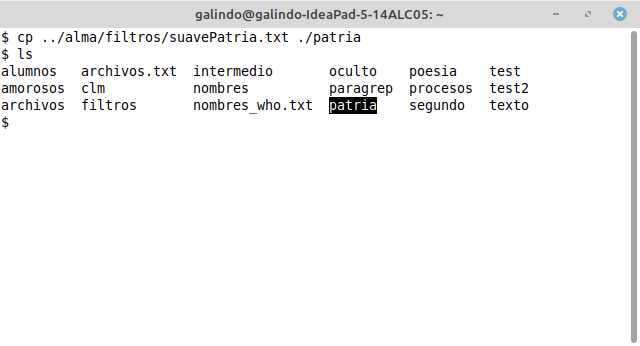
\includegraphics[width=10cm]{img/a9.png}
\caption{Archivo copiado y renombrado}
\end{figure}

\subsection{Muestre en pantalla el contenido del archivo amorosos.txt en el monitor}
\label{sec:org9bf6123}
\begin{verbatim}
cat maestro/poesia/amorosos.txt
\end{verbatim}

\begin{figure}[htbp]
\centering
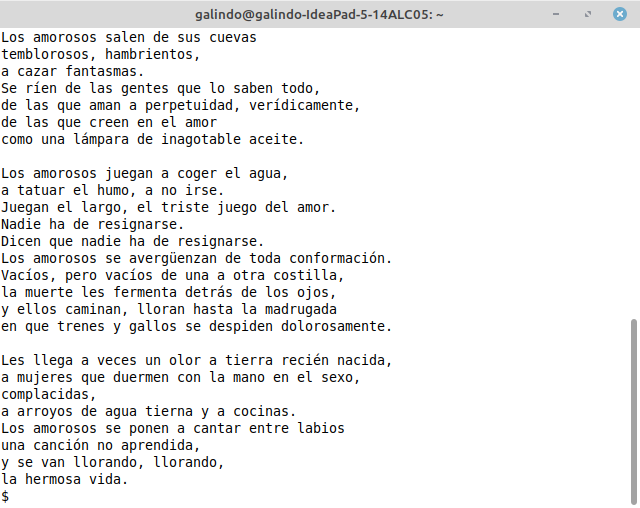
\includegraphics[width=10cm]{img/a10.png}
\caption{Contenido de amorosos.txt}
\end{figure}

\cite{linux_cat}

\subsection{Vuelva a mostrar el archivo amorosos.txt, pero por páginas}
\label{sec:org588743e}
\begin{verbatim}
more amorosos
\end{verbatim}

\begin{figure}[htbp]
\centering
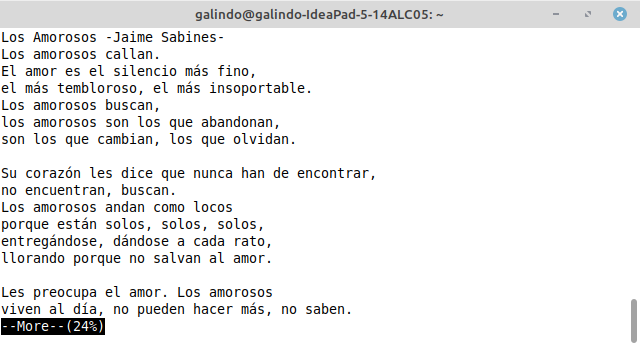
\includegraphics[width=10cm]{img/a11.png}
\caption{Presionar espacio en el teclado pasa la pagina}
\end{figure}

\subsection{Muestre las últimas diez líneas de este archivo}
\label{sec:org92abbb8}
\begin{verbatim}
tail -n 10 amorosos
\end{verbatim}

\begin{figure}[htbp]
\centering
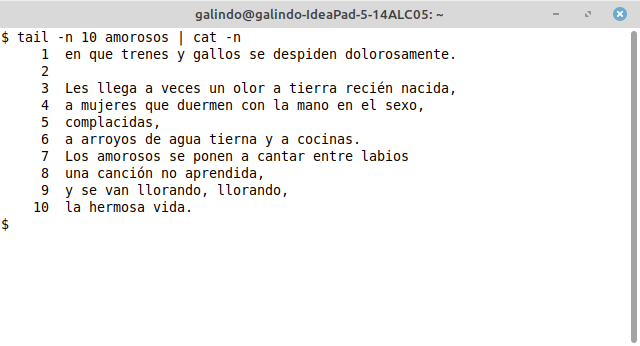
\includegraphics[width=10cm]{img/a12.png}
\caption{Ultimas 10 lineas numeradas}
\end{figure}

\pagebreak

\subsection{El archivo SuavePatria.txt ahora se llamara 'patria'}
\label{sec:org401e5f2}
\begin{verbatim}
mv ~/SuavePatria.txt ~/patria
\end{verbatim}

\begin{figure}[htbp]
\centering
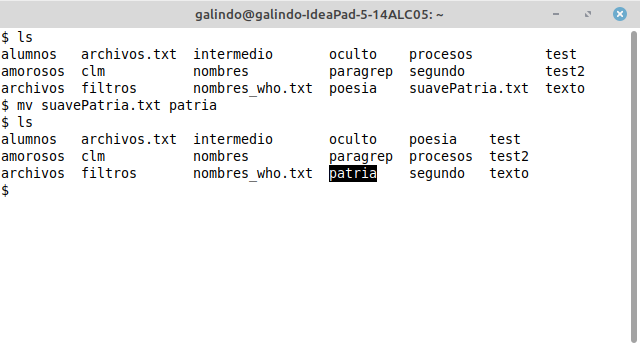
\includegraphics[width=10cm]{img/a13.png}
\caption{archivo renombrado}
\end{figure}

\subsection{Muestre las últimas ocho líneas del archivo amorosos.txt}
\label{sec:orgf261610}
\begin{verbatim}
tail -n 8 amorosos 
\end{verbatim}

\begin{figure}[htbp]
\centering
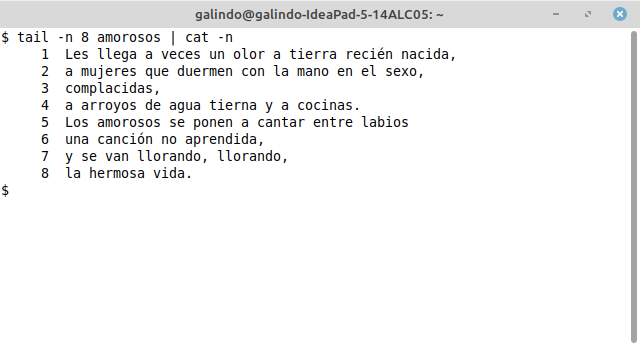
\includegraphics[width=10cm]{img/a14.png}
\caption{}
\end{figure}

\pagebreak

\subsection{¿Cuántas palabras en total contiene el archivo amorosos.txt?}
\label{sec:org5feb86a}
\begin{itemize}
\item el archivo contiene 367 palabras
\end{itemize}

\begin{verbatim}
wc -w amorosos        
\end{verbatim}

\begin{figure}[htbp]
\centering
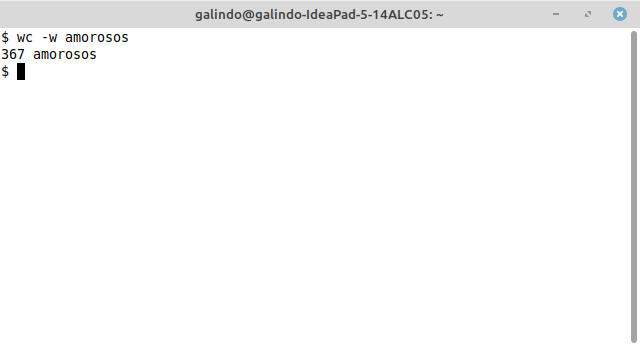
\includegraphics[width=10cm]{img/a15.png}
\caption{}
\end{figure}

\cite{linux_wc}

\subsection{¿Cuántos caracteres en total contiene el archivo Enpaz.txt?}
\label{sec:orgf463ff4}

\begin{itemize}
\item el archivo tiene 696 caracteres
\end{itemize}

\begin{verbatim}
wc -c ../alma/filtros/Enpaz.txt
\end{verbatim}

\begin{figure}[htbp]
\centering
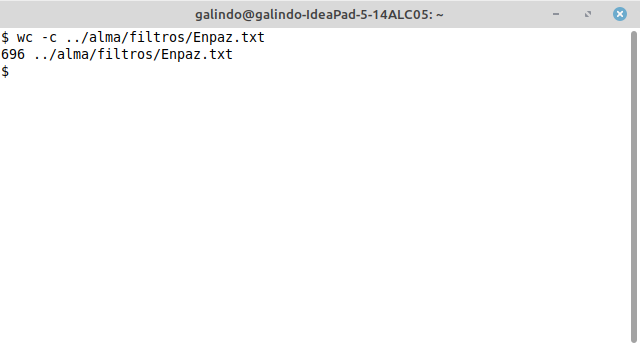
\includegraphics[width=10cm]{img/a16.png}
\caption{}
\end{figure}

\cite{linux_wc}

\subsection{Mostrar los permisos de todos los directorios que están en el directorio home}
\label{sec:org9917072}
\begin{verbatim}
cd ..
ls -l
\end{verbatim}

\begin{figure}[htbp]
\centering
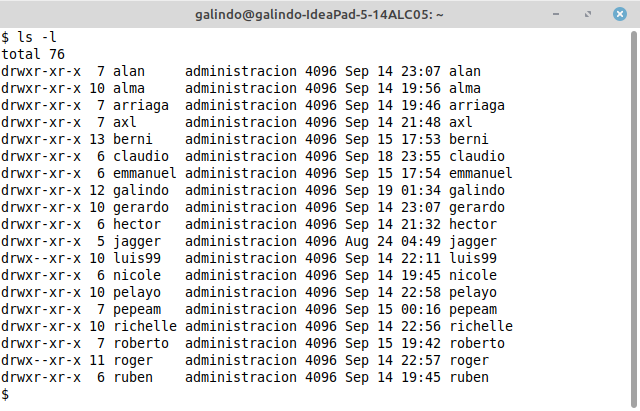
\includegraphics[width=10cm]{img/a17.png}
\caption{}
\end{figure}

\cite{linux_ls}

\subsection{Otorgue permiso a su grupo para leer y escribir en su directorio}
\label{sec:org8aa1563}
\begin{verbatim}
cd ..
chmod g+rw galindo
\end{verbatim}

\begin{figure}[htbp]
\centering
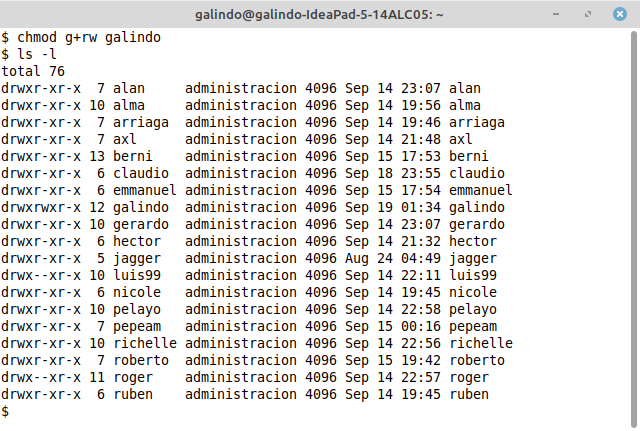
\includegraphics[width=10cm]{img/a18.png}
\caption{}
\end{figure}

\cite{linux_chmod}

\subsection{Seleccione a uno de sus compañeros, escriba un archivo en su directorio llamado 'películas' (use el comando cat). Escriba un párrafo sobre la última película que haya visto en el cine, puede ser una sinopsis o su opinión personal}
\label{sec:orge19f191}
\begin{itemize}
\item Elegí a mi compañero Héctor, por lo que para entrar a su directorio tuve que usar el siguiente comando:
\end{itemize}

\begin{verbatim}
cd ../hector/
\end{verbatim}

\begin{figure}[htbp]
\centering
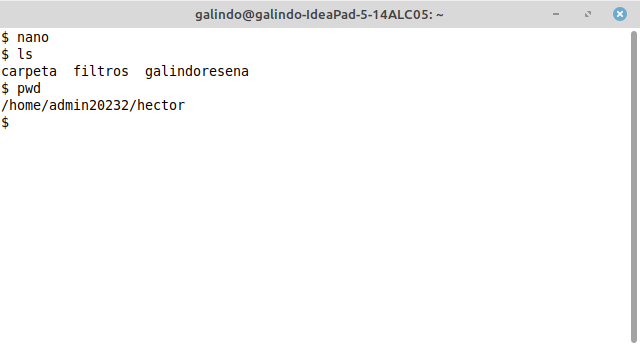
\includegraphics[width=10cm]{img/pwd.png}
\caption[\texttt{pwd}]{\texttt{pwd} para mostrar la ubicacion del directorio}
\end{figure}

Por ultimo utilice el editor nano para escribir una opinión sobre la ultima 
película que vi:

\begin{figure}[htbp]
\centering
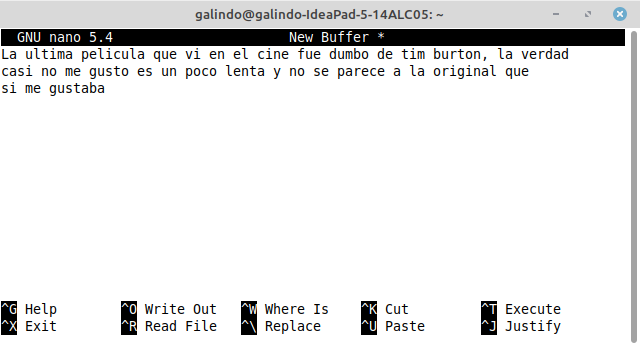
\includegraphics[width=10cm]{img/nano.png}
\caption[\texttt{nano}]{\texttt{nano} con la reseña abierta}
\end{figure}

\pagebreak

\subsection{Otorgar permiso de lectura al grupo para este archivo}
\label{sec:org42ca5c0}
\begin{verbatim}
chmod g+r galindoresena
\end{verbatim}

\begin{figure}[htbp]
\centering
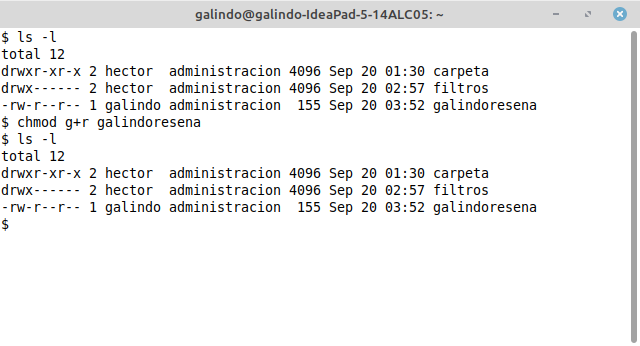
\includegraphics[width=10cm]{img/asd.png}
\caption{Permisos ajustados}
\end{figure}

\pagebreak

\subsection{Copia la historia de tres de tus compañeros a un directorio llamado 'sinopsis'}
\label{sec:org2176175}
Primero se crea el directorio con \texttt{mkdir sinopsis}

\begin{figure}[htbp]
\centering
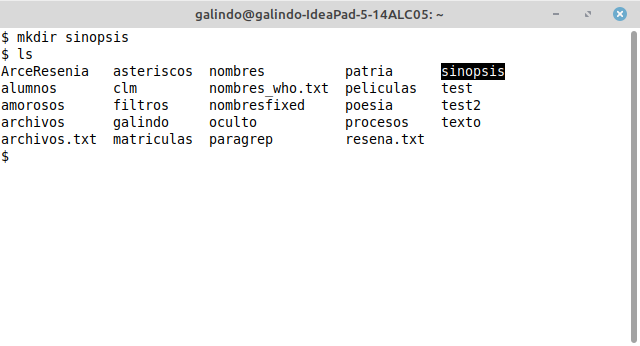
\includegraphics[width=10cm]{img/bsd.png}
\caption{directorio creado}
\end{figure}

despues de copian los archivos en el directorio 

\begin{verbatim}
cp ../hector/galindoresena\
ArceResenia\
peliculas\
sinopsis
\end{verbatim}

\begin{figure}[htbp]
\centering
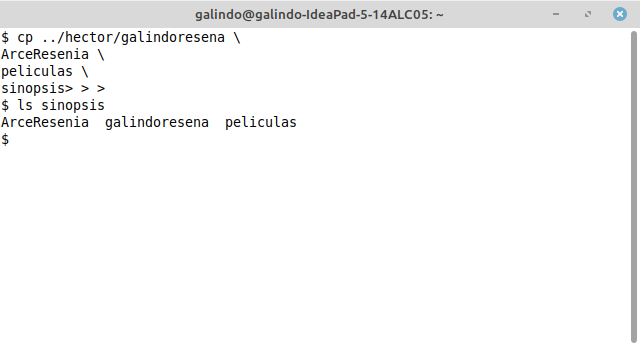
\includegraphics[width=10cm]{img/csd.png}
\caption{Archivos copiados}
\end{figure}

\pagebreak

\subsection{Restringir los permisos de lectura y escritura de su directorio al grupo}
\label{sec:org3fadf44}
\begin{verbatim}
cd ..
chmod go-rw galindo
\end{verbatim}

\begin{figure}[htbp]
\centering
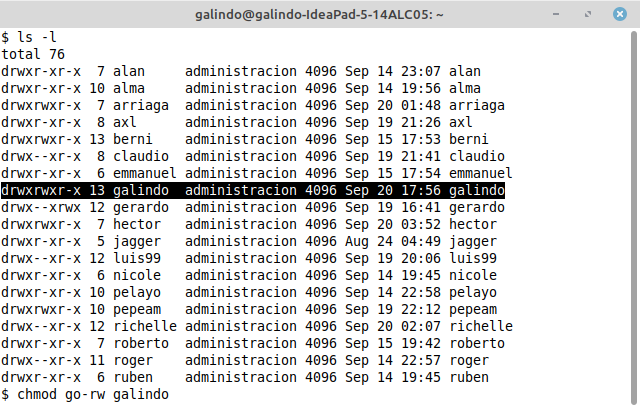
\includegraphics[width=10cm]{img/b1.png}
\caption{Lectura y escritura esta activa}
\end{figure}

\begin{figure}[htbp]
\centering
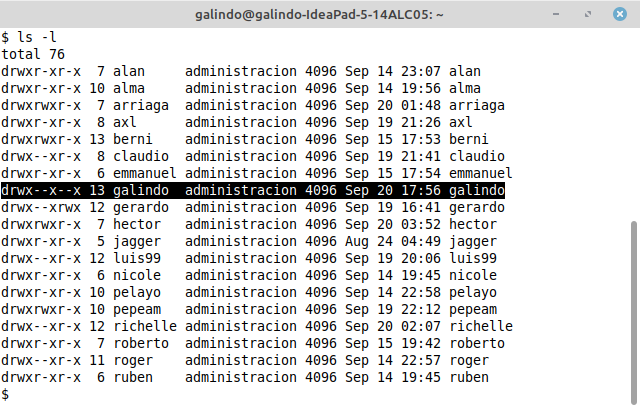
\includegraphics[width=10cm]{img/b2.png}
\caption{Lectura y escritura desactivada}
\end{figure}


\section{Conclusión}
\label{sec:orgdc04485}
A lo largo de esta practica aprendí como gestionar archivos y manipular los 
accesos que pueden tener los diferentes usuarios, pienso que conocer los 
detalles del sistema nos permitirán ser mas eficaces al momento de administrar
e interactuar con el sistema operativo y como usar las herramientas que este 
nos proporciona.

\section{Referencias}
\label{sec:org54ae829}
\printbibliography[heading=none]
\end{document}
